\documentclass{article}

\usepackage{corl_2026} % Use this for the initial submission.
% \usepackage[final]{corl_2026}
% \usepackage[preprint]{corl_2026}

\usepackage{graphicx}
\usepackage{amsmath}
\usepackage{amssymb}
\usepackage{booktabs}
\usepackage{microtype}

\title{Contact Event Gated Tactile Policies for\\In-Hand Rotation of Irregular Objects}

\author{
  Haojun Qi\\
  Department of Electrical Engineering and Computer Sciences\\
  University of California, Berkeley\\
  \texttt{rickyzhuang2003@berkeley.edu}
}

\begin{document}
\maketitle

%===============================================================================

\begin{abstract}
In-hand rotation of irregular objects requires navigating discrete contact make/break events
that fundamentally alter the local control problem. Existing tactile policies treat all
timesteps uniformly, missing the structure these events impose. We propose a
\emph{Contact-Event-Gated} (CEG) actor: a mixture-of-experts policy head in which a small
gating network conditions action selection on discretized tactile contact events, allowing the
policy to specialize distinct action strategies around contact transitions. Built on the HORA
rapid-motor-adaptation framework, the CEG policy uses a PointNet-based privileged oracle in
Stage~1 and a proprioceptive-tactile adaptation module in Stage~2, retaining full
compatibility with the existing two-stage distillation pipeline and requiring no contact regime
labels. We evaluate on 13 Branch-to-Ground (BTG) connector objects from bamboo geodesic
architecture, spanning 2-arm to 8-arm irregular geometries. The CEG policy achieves higher
rotation reward than both a proprioceptive baseline and a flat tactile policy on 11 of 13 BTG
objects, with flat tactile failing to reliably improve over the baseline without event gating.
These results suggest that the bottleneck for tactile-based dexterous manipulation of irregular
objects is not tactile information content, but architectural exploitation of contact events.
\end{abstract}

\keywords{dexterous manipulation, tactile sensing, contact events, mixture of experts, in-hand rotation}

%===============================================================================

\section{Introduction}

In-hand object rotation with a dexterous hand involves finger-gaiting: cycling fingertips
through contact-make, sustained-contact, and contact-break phases while maintaining control of
the object. This is fundamentally a hybrid control problem. Within a stable contact regime, the
appropriate joint torques are roughly continuous and predictable. At a contact event — when a
fingertip touches or releases the object — the locally optimal action map can change sharply: a
fingertip repositioning for a new grip point needs qualitatively different torques than a
fingertip sustaining force through an established contact.

Neuroscience has long recognized this structure. \citet{johansson2009} demonstrated that human
sensorimotor control uses predicted contact events as gating signals: discrete motor
subprograms are triggered at each contact phase transition, and tactile feedback from the
fingertips provides the critical early-warning signal for detecting and predicting these events
(Fig.~\ref{fig:motivation}c). Without the ability to gate behavior on contact events,
manipulation of objects with irregular geometry would be substantially impaired.

Deep RL policies for dexterous manipulation, however, do not exploit this structure
architecturally. Standard actor networks process every timestep identically, relying on the
network to implicitly discover contact-regime-conditioned behavior. Tactile observations can in
principle supply contact event information, but concatenated into a flat policy they are treated
no differently from other inputs. This problem is especially acute for irregular objects.
Symmetric objects (spheres, cylinders) have predictable contact geometry and regular
finger-gaiting cycles; irregular objects with protrusions, concavities, and asymmetric arms
force the hand through qualitatively distinct contact regimes within every grasp cycle,
demanding different action strategies at each transition.

We propose a \textbf{Contact-Event-Gated (CEG) actor}: a mixture-of-experts policy head that
explicitly conditions action selection on discretized tactile contact events. The CEG actor
maintains $K=4$ expert action heads and a small gating network. The gate reads three
contact-event features derived from current and recent tactile signals — contact force
magnitude, frame-to-frame force change, and recent mean magnitude — and produces soft mixture
weights over the experts. The final action mean is the weighted sum of expert proposals. The
gate and experts are trained end-to-end with PPO~\citep{schulman2017}; no manual contact regime
labeling is required.

We integrate the CEG actor into the HORA framework~\citep{qi2023hora}, which trains AllegroHand
in-hand rotation in two stages. Stage~1 trains a privileged oracle with ground-truth object
shape (encoded via a lightweight PointNet~\citep{qi2017pointnet}) and physical properties.
Stage~2 distills this oracle into a deployable adaptation policy that infers object properties
from proprioceptive and tactile history alone. The CEG head is used in both stages; the gate
receives only tactile observations, which are available throughout.

\begin{figure*}[t]
  \centering
  \begin{minipage}[b]{0.30\linewidth}
    \centering
    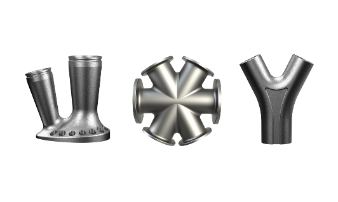
\includegraphics[width=\linewidth]{figures/Fig1a}\\[2pt]
    \small (a) BTG connector objects
  \end{minipage}
  \hfill
  \begin{minipage}[b]{0.30\linewidth}
    \centering
    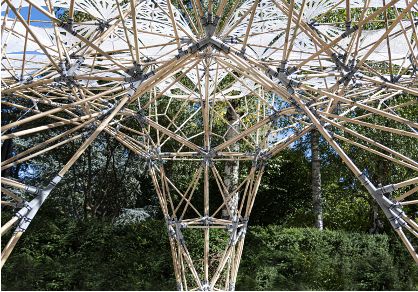
\includegraphics[width=\linewidth]{figures/Fig1b}\\[2pt]
    \small (b) Bamboo geodesic structure
  \end{minipage}
  \hfill
  \begin{minipage}[b]{0.33\linewidth}
    \centering
    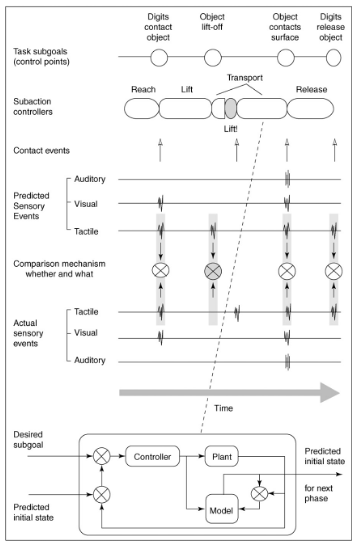
\includegraphics[width=\linewidth]{figures/Fig1c}\\[2pt]
    \small (c) Contact events gate motor subprograms \citep{johansson2009}
  \end{minipage}
  \caption{Motivation. \emph{(a)} Three representative BTG connector objects with irregular
    branching geometry. \emph{(b)} BTG connectors appear at every structural node in bamboo
    geodesic domes, embodying diverse real-world irregular shapes. \emph{(c)} In human
    sensorimotor control, contact events serve as gating signals that trigger distinct motor
    subprograms and update internal models \citep{johansson2009}. We bring this insight into
    dexterous RL policy architecture.}
  \label{fig:motivation}
\end{figure*}

We evaluate on 13 BTG connector objects (Fig.~\ref{fig:motivation}a--b) — structural nodes
from bamboo geodesic architecture — which provide a controlled and real-world-grounded benchmark
for manipulation of irregular geometries. Our main finding is that \emph{flat tactile does not
reliably improve over the proprioceptive baseline across BTG objects}, but the CEG policy
consistently outperforms both. This supports the hypothesis that the critical bottleneck is
not the presence of tactile information, but the architectural ability to exploit it at contact
events.

%===============================================================================

\section{Related Work}

\paragraph{Dexterous in-hand manipulation.}
Deep RL has enabled remarkable progress in dexterous manipulation. \citet{andrychowicz2020}
demonstrated Rubik's cube solving with a five-fingered hand through massive domain
randomization. HORA~\citep{qi2023hora} introduced rapid motor adaptation for in-hand object
rotation using a two-stage distillation pipeline; Stage~1 trains a privileged oracle and
Stage~2 produces a deployable policy that infers object properties from proprioceptive history.
\citet{chen2023visual} used visuomotor policies for reorientation of complex novel objects.
Our work extends HORA with tactile sensing and a contact-event-aware actor that operates
without visual input.

\paragraph{Tactile sensing for manipulation.}
Compact high-resolution tactile sensors~\citep{lambeta2020} have made rich fingertip feedback
practical. Tactile signals have been used for grasp stability assessment, slip detection, and
force control. For in-hand manipulation, tactile feedback is especially valuable because joint
proprioception alone provides limited contact-state information, particularly for irregular
objects where contact geometry varies rapidly. Existing tactile RL policies typically
concatenate tactile observations with proprioception in a flat network, treating contact events
as ordinary scalar inputs.

\paragraph{Mixture-of-experts and gating in RL.}
Mixture-of-experts architectures have been used in locomotion for gait transitions and in
multi-task RL for behavioral specialization. We ground our gating design in the neuroscience of
human sensorimotor control, using contact events from tactile signals as the gate variable —
distinguishing our approach from prior MoE policies that gate on task identity or motion phase.

%===============================================================================

\section{Method}
\label{sec:method}

\subsection{Base Framework: HORA}

We build on HORA~\citep{qi2023hora}, which trains AllegroHand in-hand rotation in
IsaacGym~\citep{makoviychuk2021} using 16,384 parallel environments. Stage~1 trains a
privileged PPO actor-critic with ground-truth object physics and shape encoded into an
extrinsic latent $z_t$. Stage~2 freezes the Stage~1 actor and trains a temporal convolutional
adaptation module to predict $z_t$ from proprioceptive and tactile history alone. We add
tactile observations and the CEG actor to both stages.

\subsection{Tactile Observations}

The base proprioceptive observation is a three-frame window, each frame containing 16
normalized joint positions and 16 PD targets (32D per frame, 96D total). With tactile enabled,
each frame appends a 12D contact-force vector: net contact force at all four fingertips
($4 \times 3$ xyz), scaled by $1/10$ and clipped to $[-1, 1]$, giving $3 \times 44 = 132$D.
The Stage~2 adaptation module receives a 30-frame history ($30 \times 44 = 1320$D).

\subsection{Privileged Oracle and Shape Encoding (Stage 1)}

A three-layer MLP $[256, 128, 8]$ encodes a 17D privileged physics vector (object position,
scale, mass, friction, center of mass, orientation quaternion, angular velocity) to an 8D
physics embedding $z_\text{phys}$. Object shape is encoded from a 200-point cloud by a
lightweight PointNet~\citep{qi2017pointnet} with per-point layers $[32, 32, 32]$ and global
max-pooling, yielding a 32D shape embedding $z_\text{shape}$. The oracle extrinsic is:
$z_t = [z_\text{phys} ; z_\text{shape}] \in \mathbb{R}^{40}$.

\subsection{Contact-Event-Gated Actor}

\begin{figure*}[t]
  \centering
  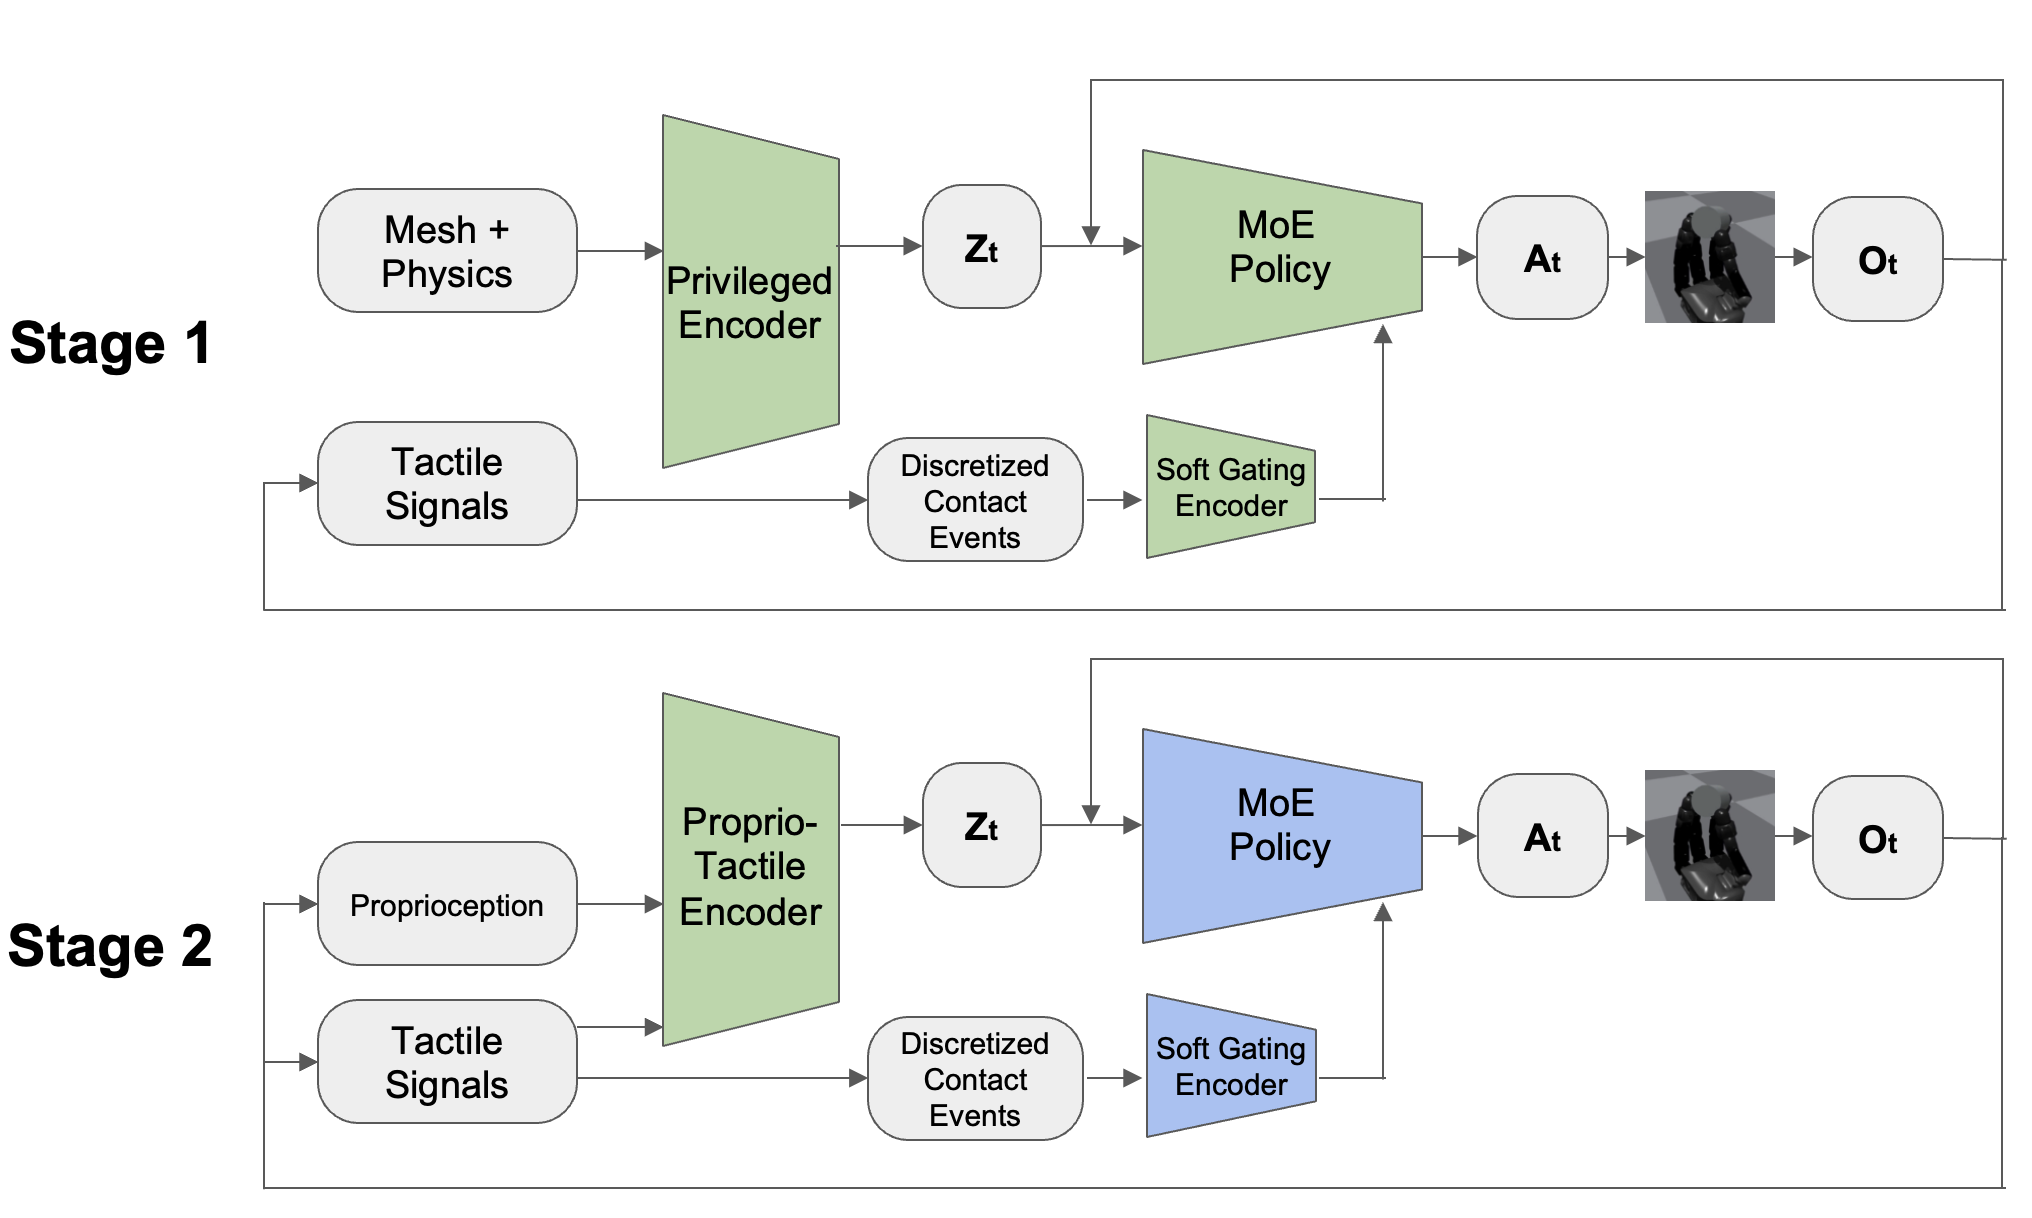
\includegraphics[width=0.88\linewidth]{figures/Fig3}
  \caption{Contact-Event-Gated (CEG) architecture. \emph{Stage~1} (top): a privileged encoder
    computes the oracle extrinsic $z_t$ from mesh and physics; a soft gating encoder reads
    discretized contact events from the tactile block and produces mixture weights; the MoE
    policy blends $K=4$ expert action heads. \emph{Stage~2} (bottom): the privileged encoder
    is replaced by a proprioceptive-tactile encoder that estimates $z_t$ from history alone;
    the CEG head and gate weights are frozen.}
  \label{fig:arch}
\end{figure*}

Fig.~\ref{fig:arch} shows the full architecture. The shared actor trunk maps the concatenated
input $[o_t ; z_t] \in \mathbb{R}^{172}$ through a three-layer MLP to a 256D feature vector
$h_t$. Four expert heads compute candidate action means:
$\mu_k = W_k h_t + b_k \in \mathbb{R}^{16}$, for $k = 1,\ldots,4$.

A small gating network reads contact-event features from the current tactile frame:
\begin{equation}
  f_t = \bigl[\,\|s_t\|_1,\;\|s_t - s_{t-1}\|_1,\;\tfrac{1}{3}
  {\textstyle\sum_{\tau=0}^{2}} \|s_{t-\tau}\|_1\,\bigr],
  \label{eq:gate_features}
\end{equation}
where $s_t \in \mathbb{R}^{12}$ is the current tactile force vector. A one-hidden-layer MLP
(32 units, ReLU) followed by a softmax maps $f_t$ to mixture weights
$w_t = (w_{t,1},\ldots,w_{t,4}) \in \Delta^3$. The final actor output is:
\begin{equation}
  \mu_t = \sum_{k=1}^{4} w_{t,k}\,\mu_k.
  \label{eq:final_action}
\end{equation}

The features in Eq.~\ref{eq:gate_features} are designed to expose the rough contact regime:
high $\|s_t\|_1$ indicates established contact; high $\|s_t - s_{t-1}\|_1$ signals a contact
event; low magnitude across all three terms indicates low or no contact. The gate and experts
are fully learned; no regime labels are provided. The critic, privileged encoder, PointNet, and
Stage~2 adaptation module are unchanged, and the CEG head is trained end-to-end with
PPO~\citep{schulman2017}.

\subsection{Stage 2 Adaptation}

Stage~2 freezes the CEG actor and trains a temporal convolutional adaptation module
$\hat{z}_t = \text{TConv}(\text{history}_{t})$ from the 30-frame proprioceptive-tactile
history. The training objective combines latent imitation and action imitation:
\begin{equation}
  \mathcal{L}_\text{adapt} = \|\hat{z}_t - z_t^*\|^2 + \|\hat{a}_t - a_t^*\|^2,
  \label{eq:adapt_loss}
\end{equation}
where $z_t^*$ and $a_t^*$ are the oracle latent and action. At deployment, the adaptation
module infers $\hat{z}_t$ and the contact gate uses the current tactile frame for $w_t$, with
both requiring only onboard sensors.

%===============================================================================

\section{Experiments}
\label{sec:experiments}

\subsection{BTG Benchmark}

\begin{figure}[t]
  \centering
  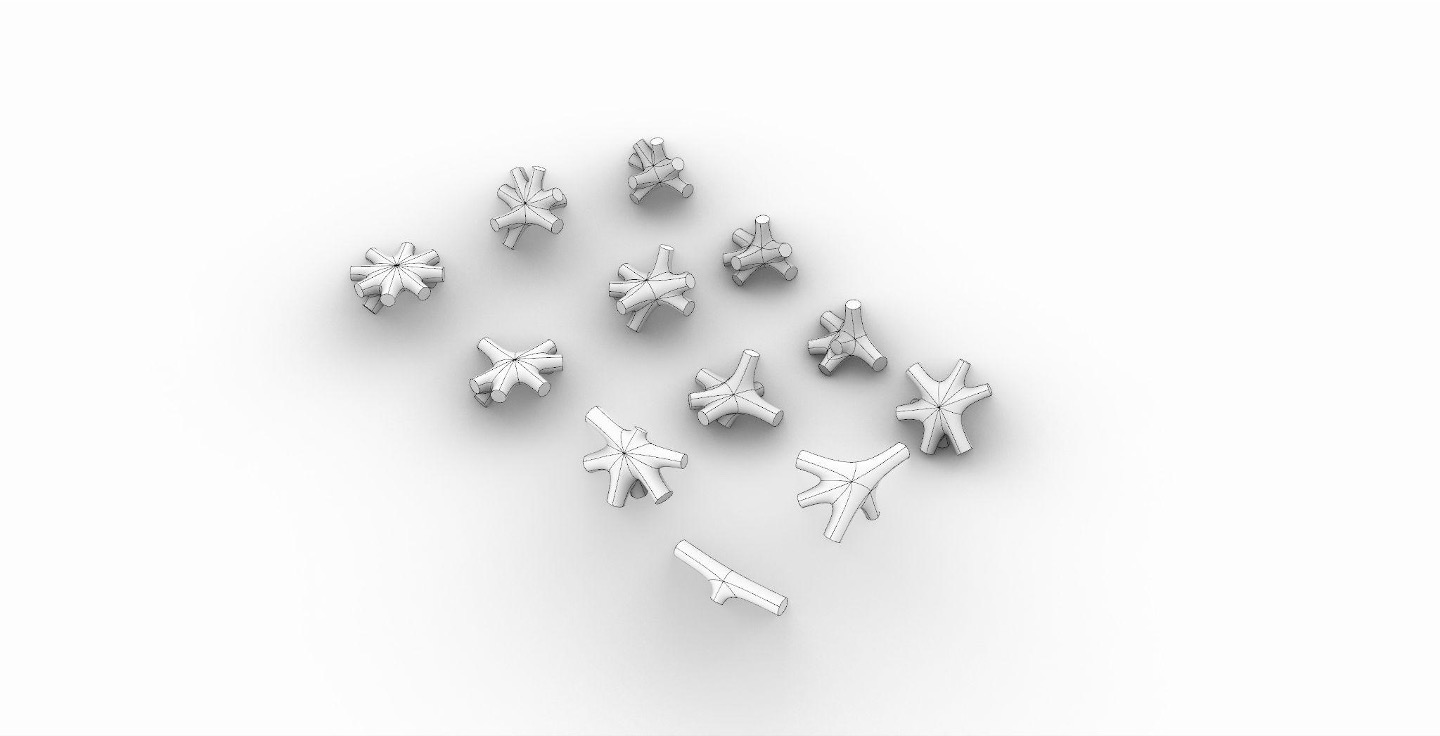
\includegraphics[width=\linewidth]{figures/Fig2}
  \caption{The 13 BTG connector objects used for evaluation, imported from 3D scans of
    structural nodes in bamboo geodesic architecture. Objects range from compact 2-arm shapes
    to complex 8-arm star geometries with no rotational symmetry.}
  \label{fig:btg}
\end{figure}

We evaluate on 13 BTG connector objects (Fig.~\ref{fig:btg}) extracted from 3D scans of
structural nodes in real bamboo geodesic domes (Fig.~\ref{fig:motivation}b). These objects
have no rotational symmetry, range from 2-arm to 8-arm branching geometries, and vary
substantially in arm count, angles, and cross-section profiles. All objects are evaluated at
the mean cylinder training scale for fair comparison; physical parameters are fixed at
randomization means during evaluation.

\subsection{Training Setup}

\begin{figure}[t]
  \centering
  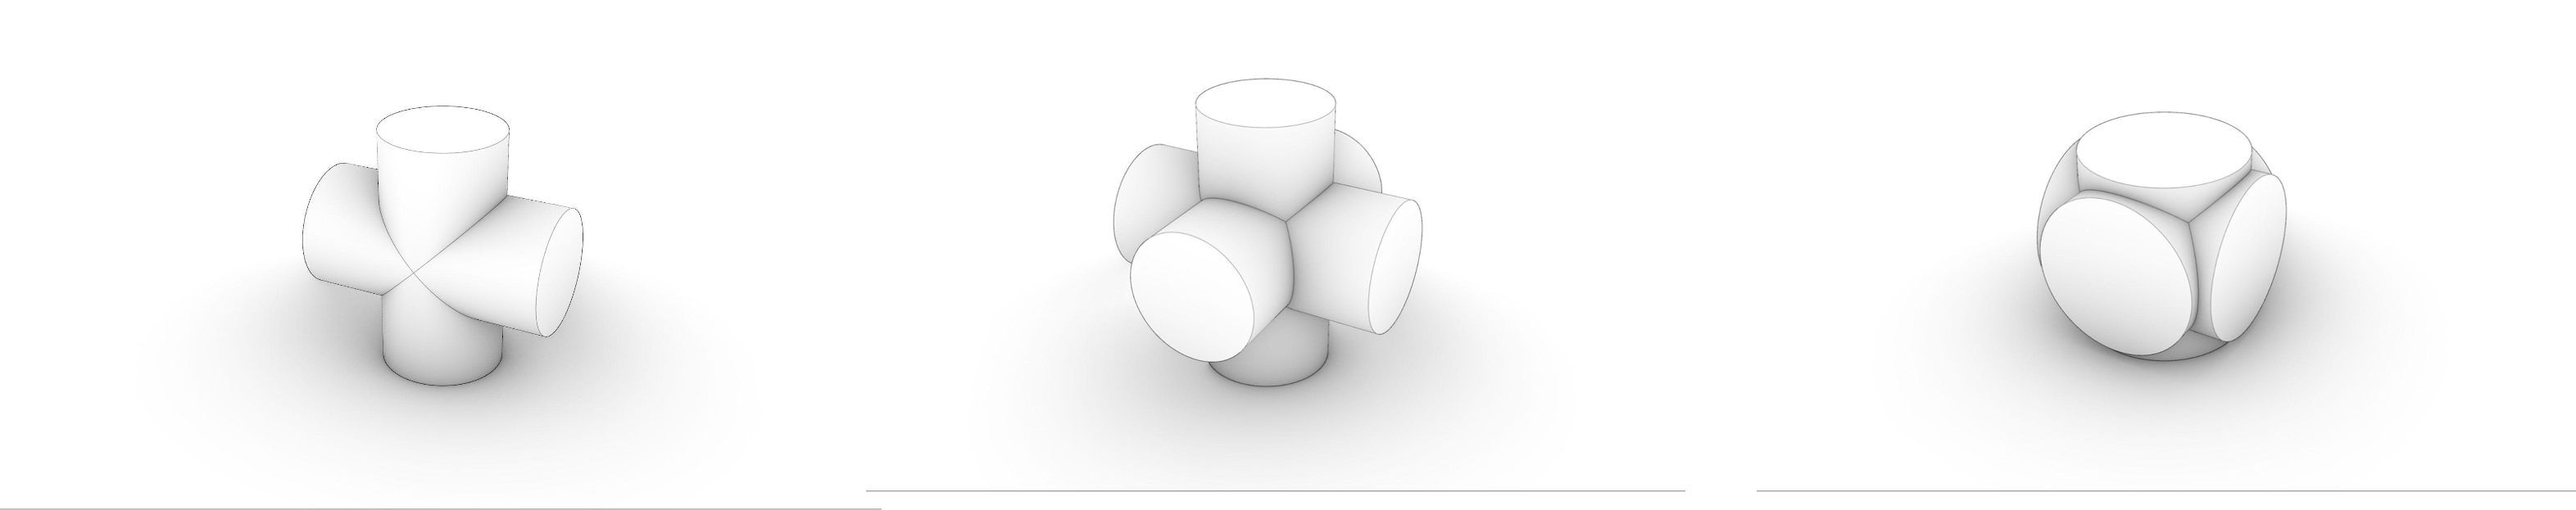
\includegraphics[width=\linewidth]{figures/Fig4a}
  \caption{Training object set: standard cylinder, 2D-cross cylinder, and 3D-cross cylinder,
    sampled with equal probability. The cross-shaped variants introduce irregular contact
    geometry without leaving the cylinder training distribution.}
  \label{fig:training}
\end{figure}

Stage~1 trains for 750M steps; Stage~2 trains for 200M steps. The training object mix includes
three cylinder variants (Fig.~\ref{fig:training}): standard cylinders, 2D-cross cylinders, and
3D-cross cylinders sampled with equal probability ($1/3$ each). Cross-shaped cylinders are
designed to expose the policy to irregular contact geometry during training while remaining
within a distribution the physics engine handles robustly. Physical parameters (mass, friction,
PD gains, scale) are randomized at training and held fixed at benchmark means for evaluation.

\subsection{Baselines}

We compare three Stage~2 policies:
\begin{itemize}\setlength\itemsep{0pt}
  \item \textbf{Baseline}: proprioceptive-only HORA Stage~2 ($96$D observation, no tactile).
  \item \textbf{Tactile}: Stage~2 with tactile appended to actor input and adaptation history
    (flat tactile, no contact gating).
  \item \textbf{Contact-Gated} (ours): Stage~2 with the CEG actor.
\end{itemize}
All three variants use the same shape-aware PointNet oracle in Stage~1 and the same temporal
convolutional architecture in Stage~2, differing only in tactile integration and actor head.

\subsection{Results and Analysis}

\begin{figure*}[t]
  \centering
  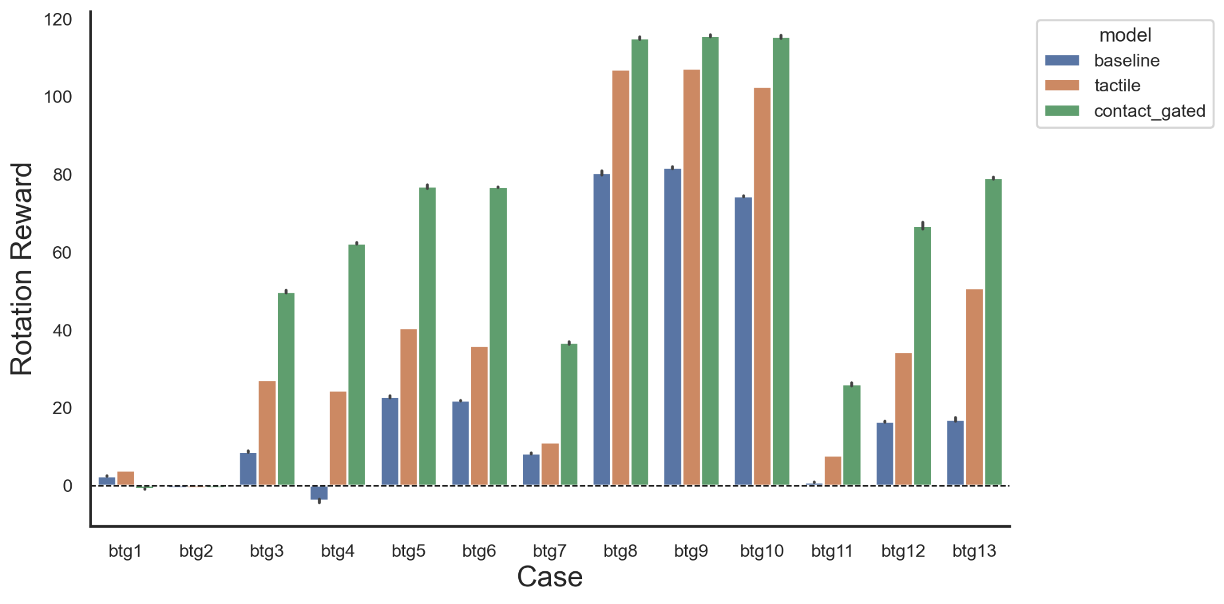
\includegraphics[width=\linewidth]{figures/Fig5}
  \caption{Rotation reward across the 13 BTG objects. The CEG policy (green) outperforms both
    the proprioceptive baseline (blue) and flat tactile policy (orange) on 11 of 13 objects.
    Flat tactile does not reliably improve over the baseline, supporting the hypothesis that
    the key bottleneck is architectural rather than informational.}
  \label{fig:results}
\end{figure*}

Fig.~\ref{fig:results} shows rotation reward across all 13 BTG objects. The CEG policy achieves
the highest reward on 11 of 13 objects.

\paragraph{Where CEG helps most.}
On moderately complex objects (btg3--btg7, btg11--btg13) — where the geometry is tractable but
requires the hand to navigate multiple distinct contact regimes per grasp cycle — the CEG policy
shows large margins over both baselines. This is consistent with the gating hypothesis: when
the hand regularly traverses qualitatively different contact states, having dedicated expert
heads per regime pays off.

\paragraph{Flat tactile does not reliably help.}
On several objects (btg7, btg11), flat tactile provides only marginal improvement over the
proprioceptive baseline, while the CEG policy shows a clear gain on the same objects. This
confirms that the issue is not the presence of tactile information but its architectural use:
raw tactile concatenated into a flat network is insufficient to unlock contact-event-conditioned
behavior.

\paragraph{Hard objects.}
On btg1 and btg2, all methods perform near zero. Inspection suggests these objects have
contact geometry far from the cylinder training distribution (very flat or elongated profiles),
making them plausible out-of-distribution cases. Extending the training object set to better
cover such geometries is a promising direction.

\paragraph{High-reward objects.}
On the most tractable objects (btg8--btg10), all methods achieve positive rotation reward. The
CEG policy still leads, but the margins are smaller, suggesting that the task is sufficiently
easy for any capable policy once the object is graspable.

%===============================================================================

\section{Conclusion}

We presented a Contact-Event-Gated (CEG) actor for dexterous in-hand rotation of irregular
objects, motivated by the neuroscientific observation that contact events gate motor subprograms
in human manipulation. By conditioning a mixture-of-experts action head on discretized tactile
contact-event features, the CEG policy consistently outperforms flat tactile and proprioceptive
baselines across 13 BTG connector objects — without contact regime labels or changes to the
two-stage RL training pipeline. Our results suggest that explicit contact event structure is a
useful inductive bias for tactile dexterous manipulation, and that the benefit of tactile
sensing depends critically on how it is used architecturally rather than merely on its
inclusion. Future work includes deployment on physical hardware with real-time tactile sensors,
extending training object diversity to cover out-of-distribution geometries, and exploration of
harder gating variants with explicit contact-event prediction as an auxiliary loss.

%===============================================================================

\clearpage
\acknowledgments{Experiments were conducted on Modal Cloud (A100 GPUs). We thank the HORA
project for the simulation infrastructure and training pipeline.}

%===============================================================================

\bibliography{report_refs}

\end{document}
